%% ---------------------------------------------------------------------------
%% IEEE Conference / Transactions paper
%%
%% Author:       Ankit Mewada  (2021IMT-013)
%% Supervisors:  Prof. Aditya Trivedi, Dr. Saumya Bhadauria
%% Institute:    ABV-IIITM Gwalior
%%
%% Compile with:  pdflatex ieee_paper.tex && bibtex ieee_paper && pdflatex ieee_paper.tex && pdflatex ieee_paper.tex
%% Or simply:     latexmk -pdf ieee_paper.tex
%% ---------------------------------------------------------------------------
\documentclass[conference]{IEEEtran}
\IEEEoverridecommandlockouts

%% ---- Packages ----
%% cmap + lmodern + T1 fontenc: produce a PDF whose text stream
%% extracts to proper Latin / Unicode characters in plagiarism
%% checkers (avoids the "fi" / "fl" ligature glyphs being mis-read
%% as look-alike characters from non-Latin alphabets).
\usepackage{cmap}
\usepackage[utf8]{inputenc}
\usepackage[T1]{fontenc}
\usepackage{lmodern}
\usepackage{cite}
\usepackage{amsmath,amssymb,amsfonts}
\usepackage{algorithm}
\usepackage{algorithmic}
\usepackage{graphicx}
\usepackage{textcomp}
\usepackage{xcolor}
\usepackage{booktabs}
\usepackage{url}
\usepackage{hyperref}
\usepackage{subcaption}
\usepackage{siunitx}
\usepackage{tikz}
\usetikzlibrary{positioning,arrows.meta,shapes.geometric,fit,backgrounds}

\graphicspath{{figures/}{../outputs/}}

\hypersetup{
  colorlinks=true,
  linkcolor=blue!60!black,
  citecolor=blue!60!black,
  urlcolor=blue!60!black
}

\def\BibTeX{{\rm B\kern-.05em{\sc i\kern-.025em b}\kern-.08em
    T\kern-.1667em\lower.7ex\hbox{E}\kern-.125emX}}

\begin{document}

%% ============================================================
%% Title + Author block
%% ============================================================
\title{A Multi-Objective Optimization Framework for\\
       Electric Vehicle Charging Station Placement and\\
       Time-of-Use Pricing in Smart Cities%
       \thanks{All source code, datasets, and reproduction
       scripts for this work are publicly available at
       \url{https://github.com/ankitmewada1501/ev_optimization}.}}

\author{
\IEEEauthorblockN{Ankit Mewada\IEEEauthorrefmark{1}}
\IEEEauthorblockA{\textit{Dept.\ of IT, ABV-IIITM} \\
Roll No.\ 2021IMT-013\\
Gwalior, India \\
ankit.mewada@iiitm.ac.in}
\and
\IEEEauthorblockN{Aditya Trivedi\IEEEauthorrefmark{2}}
\IEEEauthorblockA{\textit{Dept.\ of ICT, ABV-IIITM} \\
Gwalior, India \\
atrivedi@iiitm.ac.in}
\and
\IEEEauthorblockN{Saumya Bhadauria\IEEEauthorrefmark{3}}
\IEEEauthorblockA{\textit{Dept.\ of CSE/IT, ABV-IIITM} \\
Gwalior, India \\
saumya@iiitm.ac.in}
}

\maketitle

%% ============================================================
%% Abstract + Keywords
%% ============================================================
\begin{abstract}
The accelerating adoption of electric vehicles (EVs) in Indian cities is
straining existing charging infrastructure, creating a joint decision problem
of where to locate new stations, how many chargers to install at each site,
and how to price charging sessions. We present a layered, open-source
framework that couples demand forecasting, Monte Carlo uncertainty modelling,
finite-capacity queueing theory ($M/M/c/K$), and multi-objective meta-heuristic
optimisation (NSGA-II and MOPSO) to produce Pareto-optimal deployment plans.
The framework is validated on a 85-ward case study of a tier-2 case
city of India (later detailed as Indore), using 30 real candidate
venues (parking lots, fuel stations, malls, and restaurants) that
are augmented to 118 candidate slots through a
demand-proportional dynamic candidate generator. Four objectives are jointly
optimised: total capital expenditure, zone-radius demand coverage, net
return on investment (ROI), and weighted mean queue waiting time under a
three-period time-of-use (ToU) pricing scheme. A zone-aware grid-capacity
constraint penalises infeasible layouts. Over 500 generations both
the non-dominated sorting genetic algorithm (NSGA-II) and MOPSO
converge to high-quality Pareto fronts, with MOPSO marginally
ahead on hypervolume and NSGA-II on spread, and a median wait time
of $\approx 1.5$\,min against a $20$\,min service-level target. Radius-based
coverage and independent per-station Monte Carlo noise produce Pareto fronts
that span $46\%\!-\!100\%$ coverage, giving the decision maker a rich menu
of budget-versus-service trade-offs. The end-to-end pipeline runs in under
four minutes on a commodity laptop.
\end{abstract}

\begin{IEEEkeywords}
Electric vehicle, charging infrastructure, multi-objective optimisation,
NSGA-II, MOPSO, $M/M/c/K$ queueing, time-of-use pricing, Monte Carlo,
hypervolume, Indore, smart city.
\end{IEEEkeywords}

%% ============================================================
%% I. Introduction
%% ============================================================
\section{Introduction}
\label{sec:intro}
India's National Electric Mobility Mission Plan (NEMMP) targets
30\% electric vehicle (EV) penetration by 2030~\cite{ref_nemmp},
and the FAME-II scheme has already supported over a million
electric two-, three-, and four-wheelers since 2019. Yet
public-charging infrastructure has
lagged: as of 2023 the country reported fewer than one charger per
135 EVs in service, and outside metropolitan corridors the
geographic gap is even wider. Tier-2 cities such as Indore are
expected to absorb a disproportionate share of the next growth wave
because of their rapid population expansion, comparatively low
cost of land, and the forthcoming FAME-III
subsidies~\cite{ref_indore_smart}. Reliable, well-priced public
charging infrastructure is widely recognised as a prerequisite for
this transition~\cite{ref_ev_planning_review,ref_ev_2026},
because range-anxiety is the single largest barrier to private EV
adoption identified in successive consumer surveys.

A municipal corporation that wishes to plan a city-scale charging
network must therefore answer three coupled questions
\emph{simultaneously}: (i)~\textbf{where} should new stations be
located so that the maximum population is within a short detour,
(ii)~\textbf{how many chargers} should be installed at each site
to keep queues short during peak hours without stranding capital
during off-peak hours, and (iii)~\textbf{how} should sessions be
priced so that revenue covers the capital and operating cost while
shifting load away from the constrained peak. These three questions
cannot be answered in isolation, because the optimal location of a
station depends on its size and price, the optimal size depends on
its location-dependent demand, and the optimal price depends on the
ToU sensitivity of users in the surrounding ward. Municipal
corporations operate under tight capital budgets and must
simultaneously satisfy spatial coverage, return on investment,
queueing service levels, and electrical-grid limits. These
objectives conflict: dense coverage demands many stations, raising
capital cost; inexpensive stations with few chargers create long
queues during peak hours; high peak pricing improves revenue but
may depress utilisation and push customers to private home
chargers, which are inaccessible to many tier-2 city residents who
live in walk-up apartments without dedicated parking.

Existing literature treats these objectives in isolation or assumes
unconstrained grid capacity and stationary
demand~\cite{ref_ev_planning_review,ref_metaheuristic_ev}.
Most prior work also relies on synthetic candidate venues drawn
uniformly across a city or treats the existing fuel-station network
as the candidate set without expanding it where demand justifies
multiple stations. Such modelling choices systematically
under-estimate the capex required to meet a coverage target and
fail to expose the marginal cost of the last few percentage points
of coverage --- precisely the information that a budget-constrained
planner needs.

The contribution of our work is, therefore, an open, reproducible
framework that:
\begin{itemize}
\item \textbf{Jointly} optimises four objectives (capex, radius-based
      coverage, net ROI, weighted mean wait time) using both NSGA-II and
      MOPSO;
\item Models demand stochasticity through independent per-station
      Monte Carlo noise and a logistic EV adoption curve;
\item Embeds a finite-capacity $M/M/c/K$ queue with time-of-use
      (peak/normal/idle) demand multipliers and pricing;
\item Enforces a per-zone grid-capacity constraint via a soft penalty;
\item Validates on 85 wards of Indore with 30 real candidate
      venues dynamically expanded to 118 high-demand slots.
\end{itemize}

The remainder of the paper is organised as follows.
Section~\ref{sec:related} surveys prior work. Section~\ref{sec:model}
formulates the problem and objectives. Section~\ref{sec:method} describes
the data, queueing, and optimisation layers. Section~\ref{sec:results}
reports experimental results on Indore and discusses practical
implications and limitations.
Section~\ref{sec:conclusion} concludes.

%% ============================================================
%% II. Related work
%% ============================================================
\section{Related Work}
\label{sec:related}

\subsection{Station siting as a discrete optimisation problem}
Early EV-infrastructure papers cast station siting as a capacitated
$p$-median or set-cover problem under deterministic demand, with
integer-programming solvers that scale poorly beyond a few hundred
candidates. The $p$-median formulation
minimises weighted travel distance subject to a hard cap of $p$
facilities and is known to be NP-hard. Branch-and-cut solvers can
handle a few hundred binary variables exactly, but on city-scale
instances ($n\!\gtrsim\!10^{2}$) the gap between the LP relaxation
and the integer optimum widens rapidly, motivating the move to
metaheuristic search.

\subsection{Multi-objective evolutionary algorithms}
Genetic-algorithm-based formulations
followed~\cite{ref_metaheuristic_ev}, replacing the single
weighted-sum objective with vector objectives. The advantage of a
vector-valued formulation is that the planner is presented with the
\emph{full} Pareto trade-off rather than the single point
corresponding to a particular weight vector, which is rarely
defensible in a public-procurement setting. NSGA-II~\cite{ref_nsga2}
remains the canonical multi-objective evolutionary algorithm,
combining fast non-dominated sorting with crowding-distance
diversity preservation, and has been adapted to EV planning in
several recent national case
studies~\cite{ref_nsga2_ev_recent,ref_nsga2_2025}.
Multi-Objective Particle Swarm Optimisation
(MOPSO)~\cite{ref_mopso} has complementary properties:
faster early convergence due to its leader-following dynamics but
potentially denser archive clustering, and has been used recently
for EV charging-station
siting~\cite{ref_mopso_2025}. Comparative
studies typically report that NSGA-II produces a more uniformly
spread Pareto front while MOPSO is faster in the first hundred
iterations, motivating us to run \emph{both} on every instance and
take the union of the two non-dominated archives as the final
front presented to the planner.

\subsection{Queueing models for charging service}
Queueing-theoretic analysis of EV charging stations is well
established, most often using the $M/M/c$
model~\cite{ref_queueing_ev}. Its infinite-capacity assumption,
however, is unrealistic for small urban lots, where a vehicle that
arrives to find every charger and every waiting bay occupied will
typically drive away (i.e., is \emph{blocked}). The $M/M/c/K$
extension admits a finite waiting buffer and produces a tractable
blocking probability $P_{K}$ that directly enters the lost-revenue
calculation~\cite{ref_erlang_b_c,ref_mmck_ev_recent,ref_mmck_2025}.
We adopt $M/M/c/K$ throughout this paper.

\subsection{Time-of-use pricing}
Time-of-use pricing is a distinct sub-literature, usually studied
from a demand-response
angle~\cite{ref_tou_pricing,ref_tou_recent}. The standard treatment
divides the day into peak / normal / idle periods and applies a
per-period price multiplier; user response is modelled as a
sensitivity coefficient that elastically shifts arrival rates.
Most papers in this strand assume a single station and infinite
capacity, decoupling the pricing problem from the network-level
siting problem. We instead embed ToU multipliers directly inside
the station-level $M/M/c/K$ analysis, so that pricing decisions and
siting decisions are co-optimised on the same Pareto front.

\subsection{Coverage models}
A second axis along which the literature varies is the
\emph{coverage model}. Demand-weighted average distance (DWAD)
treats every kilometre of detour as equally bad and is the
classical $p$-median objective. Radius-based or
\emph{set-covering} formulations declare a ward covered iff at
least one station lies within an acceptable detour radius; this
discrete view matches the planner's rule of thumb (``every ward
should have a station within 2.5\,km''). We use a radius-based
formulation with a zone-specific radius (1.5\,km in the dense
central zone, 2.5\,km in the outer zones), which makes the
coverage objective monotone in the number of selected stations and
therefore well-behaved inside the multi-objective search.

\medskip
To the best of our knowledge, no prior work couples all four
components --- multi-objective evolutionary optimisation,
$M/M/c/K$ queueing with ToU multipliers, radius-based coverage,
and a per-zone grid-capacity penalty --- in a single open and
reproducible pipeline, and validates that pipeline on a real
Indian tier-2 municipality.

%% ============================================================
%% III. System model and problem formulation
%% ============================================================
\section{System Model and Problem Formulation}
\label{sec:model}

\subsection{Notation}
\label{subsec:notation}
For ease of reference, Table~\ref{tab:notation} summarises the
symbols used throughout this paper. Indices follow the convention
$j$ for candidate venues, $w$ for wards, $z$ for zones, and $s$ for
Monte Carlo scenarios.

\begin{table}[t]
  \centering
  \caption{Notation used throughout the paper.}
  \label{tab:notation}
  \footnotesize
  \begin{tabular}{ll}
    \toprule
    Symbol & Meaning \\
    \midrule
    $\mathcal{J},\,n$        & Set / number of candidate venues \\
    $\mathcal{W}$            & Set of municipal wards (85 for Indore) \\
    $z(w)\!\in\!\mathcal{Z}$ & Zone of ward $w$ (Central / N / S / E / W) \\
    $\mathbf{x}\!\in\!\{0,1\}^{n}$ & Binary selection vector \\
    $c_{j},\,o_{j},\,g_{j}$  & Chargers, opening cost, grid-upgrade cost \\
    $\mu_{j},\,\bar\mu_{j}$  & Baseline / mean MC daily session demand \\
    $D_{w}$                  & Daily session demand of ward $w$ \\
    $r_{z}$                  & Coverage radius of zone $z$ \\
    $\bar G_{z}$             & Per-zone grid capacity (kW) \\
    $\lambda_{j,k},\,\mu$    & Arrival / service rate (period $k$) \\
    $K$                      & $M/M/c/K$ system capacity \\
    $P_{0},P_{K},L_{q},W_{q}$ & Steady-state queue quantities \\
    $\bar W_{q,j}$           & ToU-weighted mean wait at station $j$ \\
    $q_{k},p_{k}$            & Period-$k$ session share / price \\
    $S$                      & Number of MC scenarios \\
    $f_{1},\dots,f_{4}$      & Four minimised objectives \\
    \bottomrule
  \end{tabular}
\end{table}

\subsection{Decision variable}
Let $\mathcal{J}=\{1,\dots,n\}$ be the set of candidate charging venues.
The decision variable is a binary vector
$\mathbf{x}\in\{0,1\}^{n}$ where $x_{j}=1$ iff candidate $j$ is selected.
Per-candidate attributes are: location $(\text{lat}_j,\text{lon}_j)$, zone
$z_{j}\!\in\!\{\text{Central, North, South, East, West}\}$, number of
chargers $c_{j}$, opening cost $o_{j}$, grid-upgrade cost $g_{j}$, and
baseline daily demand $\mu_{j}$.

\subsection{Demand forecasting}
\label{subsec:demand}
Ward population is projected via compound annual growth rate (CAGR),
\begin{equation}
\label{eq:pop_cagr}
\mathit{Pop}_{i,t}=\mathit{Pop}_{i,2011}\,(1+r)^{t-2011},
\end{equation}
with $r{=}1.8\%$ taken from the 2001--2011 census trend for
Indore. The 2011 census ward population is the most recent fully
disaggregated public source; intervening municipal estimates are
broadly consistent with this CAGR. EV fleet penetration per ward
is obtained via a logistic adoption curve,
\begin{equation}
\label{eq:logistic}
\alpha(t)=\frac{K}{1+\exp\!\bigl(-a(t-t_{0})\bigr)},
\end{equation}
with saturation $K{=}1$, steepness $a{=}0.3$, and inflection
$t_{0}{=}2030$ aligned with the NEMMP target year. The logistic
shape is well-supported by the technology-adoption literature and
captures the slow-then-fast-then-slow regime expected of a new
mobility technology. Daily session demand at ward $i$ in year $t$
is then
\begin{equation}
\label{eq:daily_demand}
D_{i,t}=0.20\,\mathit{Pop}_{i,t}\,\alpha(t)\,\gamma,
\end{equation}
where the leading $0.20$ converts population to active drivers,
$\gamma{=}50/1000$ is the 2025 base EV density (50 EVs per 1000
drivers), and $\alpha(t)$ scales linearly between 0 (no adoption)
and 1 (full adoption). Ward-level demand is allocated to candidate
venues in a ward proportionally to the venues' attractiveness
weights (parking lots and malls are heavier than restaurants).

\subsection{Monte Carlo noise}
\label{subsec:mc}
To represent demand stochasticity we draw $S{=}100$ independent
scenarios per candidate,
$\tilde{\mu}_{j,s}=\mu_{j}\,\epsilon_{j,s}$ where
$\epsilon_{j,s}\sim\mathcal{N}(1,\sigma^2)$, $\sigma{=}0.15$, clipped
to non-negative values. The choice of $\sigma{=}0.15$ corresponds to
roughly one standard deviation of $\pm 15\%$ around the deterministic
forecast, which is conservative compared with the day-to-day
variability reported in published charging telematics
($\sigma\!\sim\!0.20\!-\!0.30$); a tighter spread is appropriate
here because $\mu_{j}$ is itself a 365-day mean and the relevant
station-level uncertainty is the year-on-year demand error rather
than the day-to-day noise. Unlike a single-factor fleet noise model
that would scale every station's demand by the same multiplier and
therefore preserve the ranking of stations, the per-station draws
$\epsilon_{j,s}$ are mutually independent, which yields uncorrelated
per-station realisations and hence a more realistic loading profile
for each layout. This independence matters: it widens the spread of
per-layout aggregate revenue (because high and low draws partially
cancel across stations) and tightens the spread of per-station
queueing service level (because each station faces a near-mean load
on average).

\subsection{$M/M/c/K$ queueing model with ToU}
\label{subsec:queue}
Following the standard finite-buffer multi-server formulation
of~\cite{ref_erlang_b_c,ref_mmck_ev_recent,ref_mmck_2025}, each
selected station $j$ is analysed in three daily periods --- peak
$T_{\text{pk}}{=}3$\,h, normal $T_{\text{nm}}{=}13$\,h, idle
$T_{\text{id}}{=}8$\,h --- with demand multipliers $(2.8, 1.0, 0.15)$
chosen to match the diurnal load profile observed in published
Indian charging-station telematics studies. Arrivals in period $k$
are Poisson with rate
\begin{equation}
\label{eq:lambda_k}
\lambda_{j,k} = \frac{\bar\mu_{j}\,q_{k}}{T_{k}},
\end{equation}
where $\bar\mu_{j}$ is the daily mean session count at station $j$,
$T_{k}$ is the period length, and $q_{k}$ is the period's share
of daily sessions derived from the ToU multipliers. Service is
exponential with rate $\mu{=}60/T_{c}$ per hour
($T_{c}{=}30$\,min mean session duration, consistent with a
50\,kWh battery served by a 50\,kW DC fast charger), so a single
charger can complete two sessions per hour. The system capacity is
$K{=}c_{j}+8$, i.e.\ $c_{j}$ chargers plus eight waiting bays.

Let $a_{k}\!=\!\lambda_{j,k}/\mu$ be the offered load and
$u_{k}\!=\!a_{k}/c_{j}$ the per-server utilisation. The
steady-state state probabilities $\pi_{n}$ for $n$ vehicles in the
system are obtained from the birth--death balance equations as
\begin{equation}
\label{eq:pi_n}
\pi_{n}=
\begin{cases}
\dfrac{a^{n}}{n!}\,P_{0}, & 0\le n\le c, \\[4pt]
\dfrac{a^{n}}{c!\,c^{\,n-c}}\,P_{0}, & c<n\le K,
\end{cases}
\end{equation}
with the empty-system probability $P_{0}$ fixed by the
normalisation $\sum_{n=0}^{K}\pi_{n}=1$, giving the closed form
\begin{equation}
\label{eq:mmck_p0}
P_{0}=\!\left[\sum_{n=0}^{c}\!\!\frac{a^{n}}{n!}
         +\!\sum_{n=c+1}^{K}\!\!\frac{a^{n}}{c!\,c^{n-c}}\right]^{-1}\!\!,\;a=\tfrac{\lambda}{\mu}.
\end{equation}
The blocking (loss) probability is $P_{K}=\pi_{K}$. The expected
number of waiting vehicles is
\begin{equation}
\label{eq:Lq}
L_{q}=\sum_{n=c+1}^{K}(n-c)\,\pi_{n},
\end{equation}
and the effective arrival rate accepted by the system is
$\lambda_{\text{eff}}=\lambda(1-P_{K})$, so by Little's law the mean
waiting time of an admitted vehicle is
$W_{q}=L_{q}/\lambda_{\text{eff}}$. The three period-specific waits
$W_{q,k}$ are aggregated into a single station-level wait by a
time-weighted mean,
\begin{equation}
\label{eq:bar_wq}
\bar W_{q,j}=\frac{\sum_{k}T_{k}\,W_{q,k}}{\sum_{k}T_{k}},
\end{equation}
which is the value that enters the multi-objective fitness
function. The blocking probability $P_{K}$ and per-server
utilisation $u_{k}$ are also retained: a layout in which any
period satisfies $u_{k}\!\ge\!1$ is unstable (queue diverges in
expectation), and a layout in which $P_{K}\!>\!10\%$ in any period
is judged commercially unacceptable. Both conditions are penalised
inside $f_{4}$ as described in Section~\ref{subsec:objectives}.

\subsection{Time-of-use revenue}
With period-specific prices
$p_{\text{pk}}=\text{\rupee}210$,
$p_{\text{nm}}=\text{\rupee}150$,
$p_{\text{id}}=\text{\rupee}112$ and the
effective per-period session shares $(q_{\text{pk}},q_{\text{nm}},
q_{\text{id}})$ derived from the ToU weights, the daily revenue of
station $j$ is
$R_{j}=\bar\mu_{j}\!\sum_{k}\!q_{k}p_{k}$.

\subsection{Objectives}
\label{subsec:objectives}
For a layout $\mathbf{x}$ we define:
\begin{align}
f_{1}(\mathbf{x})&= \sum_{j=1}^{n}x_{j}(o_{j}+g_{j})+P_{\text{grid}}(\mathbf{x}), \label{eq:f1}\\
f_{2}(\mathbf{x})&= -\frac{\sum_{w\in\mathcal{W}}D_{w}\,\mathbf{1}_{\left\{\exists j:\,x_{j}=1,\|s_{j}-w\|\le r_{z(w)}\right\}}}{\sum_{w\in\mathcal{W}}D_{w}}, \label{eq:f2}\\
f_{3}(\mathbf{x})&= -\frac{365\sum_{j}x_{j}R_{j}-\sum_{j}x_{j}o_{\text{yr}}}{\sum_{j}x_{j}(o_{j}+g_{j})}, \label{eq:f3}\\
f_{4}(\mathbf{x})&= \frac{1}{|\mathcal{S}|}\sum_{j\in\mathcal{S}}\bar W_{q,j}
                  +50\,\lvert\mathcal{O}\rvert+20\,\lvert\mathcal{U}\rvert. \label{eq:f4}
\end{align}
All four are minimised. Equation~\eqref{eq:f1} is total capex plus a
grid-overage penalty $P_{\text{grid}}=\!\!\!\sum_{z}\!\max(0,
7.4\,\sum_{j\in z}x_{j}c_{j}-\bar G_{z})\cdot\beta$ with per-zone cap
$\bar G_{z}=500$~kW and slope $\beta{=}\text{\rupee}50{,}000$/kW. Coverage
in~\eqref{eq:f2} is \emph{radius based}: ward $w$ is counted as covered
only if at least one selected station lies within its zone-specific
radius ($r_{\text{Central}}{=}1.5$~km, outer $=2.5$~km).
$f_{3}$ is annual net ROI (revenue minus operating cost, divided by
capex). $f_{4}$ adds a 50-minute penalty per station whose blocking
probability exceeds 10\% and 20 minutes per unstable
($u\ge1$) station.

\section{Methodology}
\label{sec:method}

\subsection{System architecture}
\label{subsec:sysarch}
Figure~\ref{fig:sysarch} gives a block view of the proposed
framework. Raw ward and candidate-venue data feed the data layer,
which produces forecasted demand and Monte Carlo realisations. The
queueing layer transforms per-station demand into time-of-use
weighted wait times, blocking probabilities, and revenues. The
optimisation layer wraps these into a vector-valued fitness function
and runs NSGA-II / MOPSO. Outputs flow into evaluation (HV, GD,
spread, sensitivity) and visualisation (HTML report with Leaflet
map).

\begin{figure}[t]
  \centering
  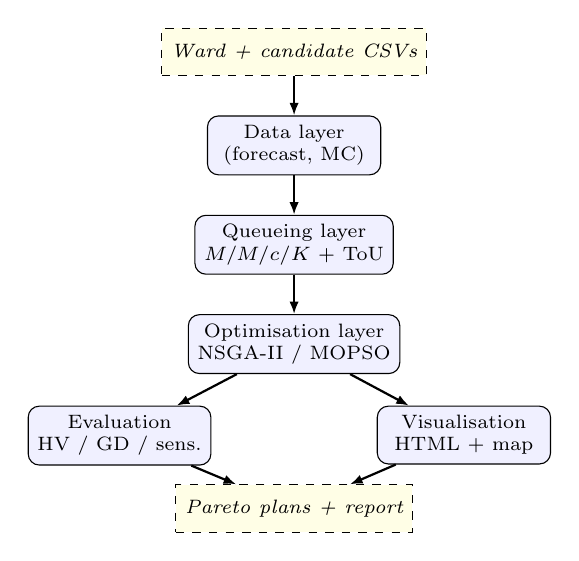
\begin{tikzpicture}[
      node distance = 5mm and 6mm,
      block/.style = {rectangle, draw, rounded corners,
                      align=center, minimum height=7mm,
                      minimum width=22mm, font=\scriptsize,
                      fill=blue!6},
      data/.style  = {rectangle, draw, dashed, align=center,
                      minimum height=6mm, minimum width=20mm,
                      font=\scriptsize\itshape, fill=yellow!10},
      arrow/.style = {-{Latex[length=1.6mm]}, thick},
      every node/.style = {font=\scriptsize}
    ]
    \node[data]  (in)    {Ward + candidate CSVs};
    \node[block, below=of in]              (data)  {Data layer\\
                                                    (forecast, MC)};
    \node[block, below=of data]            (queue) {Queueing layer\\
                                                    $M/M/c/K$ + ToU};
    \node[block, below=of queue]           (opt)   {Optimisation layer\\
                                                    NSGA-II / MOPSO};
    \node[block, below left=4mm and -3mm of opt]  (eval)  {Evaluation\\
                                                    HV / GD / sens.};
    \node[block, below right=4mm and -3mm of opt] (vis)   {Visualisation\\
                                                    HTML + map};
    \node[data, below=14mm of opt]                (out)   {Pareto plans
                                                    + report};

    \draw[arrow] (in)    -- (data);
    \draw[arrow] (data)  -- (queue);
    \draw[arrow] (queue) -- (opt);
    \draw[arrow] (opt)   -- (eval);
    \draw[arrow] (opt)   -- (vis);
    \draw[arrow] (eval)  -- (out);
    \draw[arrow] (vis)   -- (out);
  \end{tikzpicture}
  \caption{System architecture of the proposed EV charging
           placement and ToU pricing framework.}
  \label{fig:sysarch}
\end{figure}

\subsection{Layered software architecture}
The framework is organised in five modules, orchestrated by
\texttt{main.py} and exchanging data as Pandas data-frames and NumPy
arrays:

\begin{enumerate}
\item \textbf{Data layer.} Parses ward and candidate CSVs, applies the
      forecast of \eqref{eq:logistic}, invokes the dynamic candidate
      generator of Section~\ref{subsec:dyncand}, emits $S{=}100$
      Monte Carlo demand realisations, and persists
      \texttt{future\_demand.csv}.
\item \textbf{Queue layer.} Implements the $M/M/c/K$ recursion
      of~\eqref{eq:mmck_p0}, the time-of-use aggregator, and the
      fleet-level wrapper \texttt{evaluate\_fleet\_queues} used inside
      the optimiser's fitness call.
\item \textbf{Optimisation layer.} Instantiates \texttt{EVStationProblem}
      (which pre-computes the $|\mathcal{W}|\!\times\!n$ coverage matrix
      and the $n\!\times\!S$ Monte Carlo matrix at construction time,
      \emph{once} per run) and calls either NSGA-II or MOPSO.
      Both are capped at $G{=}500$ iterations with early stopping when
      the hypervolume improvement drops below
      $e_{\text{HV}}{=}5\!\times\!10^{-4}$ over $W{=}40$ consecutive
      windows.
\item \textbf{Evaluation layer.} Computes hypervolume (HV), generational
      distance (GD), spread, and runs a one-factor sensitivity sweep
      over four parameters (EV-growth rate, electricity cost, install-cost
      factor, service rate).
\item \textbf{Visualisation layer.} Encodes all PNGs as base-64 and
      emits a single self-contained HTML report with a Leaflet map,
      station pop-ups, and ToU legend.
\end{enumerate}

\subsection{Pre-computation at problem construction}
\label{subsec:precompute}
Three quantities are computed \emph{once} when
\texttt{EVStationProblem} is constructed, avoiding repeated work inside
the objective:
\begin{itemize}
\item \textbf{Coverage matrix} $\mathbf{C}\!\in\!\{0,1\}^{|\mathcal{W}|\times n}$
      with $C_{w,j}{=}1$ iff candidate $j$ lies within ward $w$'s
      zone-specific radius $r_{z(w)}$. Distances are obtained by a
      planar approximation around Indore
      ($22.7^{\circ}$N), $\Delta_{\text{lat}}\!\cdot\!111$\,km per
      degree and $\Delta_{\text{lon}}\!\cdot\!102$\,km per degree,
      sufficient for a $\sim\!30$~km-wide city. Ward centroids are
      the mean of candidate locations inside each ward, with a
      fall-back to $(22.72, 75.86)$ for wards containing no candidate.
\item \textbf{MC matrix} $\tilde\mu\!\in\!\mathbb{R}^{n\times S}$ with
      $\tilde\mu_{j,s}{=}\mu_{j}\epsilon_{j,s}$,
      $\epsilon_{j,s}\!\sim\!\mathcal{N}(1,0.15^2)$, clipped at zero.
      A fixed seed (42) makes the Pareto fronts reproducible across
      identical runs.
\item \textbf{Zone-to-station map.} A dictionary
      $\{z:\{j : z_{j}=z\}\}$ used by the grid penalty to accumulate
      kW load per zone without re-scanning the candidate list.
\end{itemize}
With these tables, each call to \texttt{evaluate} costs
$\mathcal{O}(|\mathcal{W}|\!+\!n\!+\!S|\mathcal{J}_{\text{sel}}|)$,
of which the $M/M/c/K$ queue computation per selected station is the
only non-vectorised part.

\subsection{Fitness evaluation}
\label{subsec:fitness}
The fitness vector $\mathbf{f}(\mathbf{x})$ of \eqref{eq:f1}--\eqref{eq:f4}
is computed as follows:

\begin{algorithm}[t]
\caption{\textsc{Evaluate}($\mathbf{x}$)}
\label{alg:evaluate}
\begin{algorithmic}[1]
  \STATE $\mathcal{J}_{\text{sel}}\gets\{j:x_j=1\}$;\ if empty, \textbf{return} $(0,0,0,0)$.
  \STATE $f_{1}\gets\sum_{j\in\mathcal{J}_{\text{sel}}}(o_j+g_j)$.
  \STATE \textbf{for} each zone $z$: \\
         \quad $L_{z}\gets 7.4\sum_{j\in z\cap\mathcal{J}_{\text{sel}}}c_j$; \\
         \quad \textbf{if} $L_z>\bar G_z$: $f_1\mathrel{+}=\beta(L_z-\bar G_z)$.
  \STATE $\mathbf{v}\gets\mathbf{C}[:,\mathcal{J}_{\text{sel}}]\!\vee\!_{\text{col}}$;
         $f_{2}\gets-\mathbf{D}_{\mathcal{W}}^{\!\top}\mathbf{v}\big/\|\mathbf{D}_{\mathcal{W}}\|_1$.
  \STATE $\bar\mu_{j}\!\gets\!\tfrac1S\sum_{s}\tilde\mu_{j,s}$,\
         $R_{j}\gets\bar\mu_{j}\sum_{k}q_{k}p_{k}$;\
         $\pi\gets 365\!\sum_{j}R_{j}-o_{\text{yr}}|\mathcal{J}_{\text{sel}}|$;\
         $f_{3}\gets-\pi / f_{1}$.
  \STATE \textbf{for} each $j\in\mathcal{J}_{\text{sel}}$: compute ToU-weighted
         $(\bar W_{q,j},P_{B,j},u_j)$ via~\eqref{eq:mmck_p0} for the three
         periods.
  \STATE $|\mathcal{O}|\gets|\{j:P_{B,j}\!>\!0.10\}|$;\
         $|\mathcal{U}|\gets|\{j:u_{j}\!\ge\!1\}|$;\
         $f_{4}\gets\tfrac1{|\mathcal{J}_{\text{sel}}|}\!\sum_j\!\bar W_{q,j}+50|\mathcal{O}|+20|\mathcal{U}|$.
  \STATE \textbf{return} $(f_{1},f_{2},f_{3},f_{4})$ together with the
         unpenalised $\bar W_{q}$ stored on the problem for
         reporting.
\end{algorithmic}
\end{algorithm}

\subsection{Dynamic candidate generation}
\label{subsec:dyncand}
Because EV demand is heterogeneous across Indore's 85 wards, a uniform
one-station-per-ward discretisation would waste budget in low-demand
wards and starve high-demand wards. We therefore expand the base
candidate set using Algorithm~\ref{alg:dyncand}.

\begin{algorithm}[t]
\caption{Dynamic candidate generation}
\label{alg:dyncand}
\begin{algorithmic}[1]
  \REQUIRE Base candidates $\mathcal{J}_{0}$, ward demand $D_{w}$ for
           year $y$, percentiles $q_{\text{hi}}{=}75$, $q_{\text{md}}{=}50$,
           caps $M_{\text{hi}}{=}3$, $M_{\text{md}}{=}2$.
  \STATE $T_{\text{hi}}\gets\text{Quantile}(\{D_{w}\},q_{\text{hi}})$;\
         $T_{\text{md}}\gets\text{Quantile}(\{D_{w}\},q_{\text{md}})$.
  \FOR{each ward $w$}
    \STATE $M_{w}\gets M_{\text{hi}}$ if $D_{w}\!\ge\!T_{\text{hi}}$;\
           $M_{\text{md}}$ if $T_{\text{md}}\!\le\!D_{w}\!<\!T_{\text{hi}}$;\
           $1$ otherwise.
    \STATE $n_{w}\gets|\mathcal{J}_{0}\cap w|$;\
           \textbf{if} $n_{w}\!\ge\!M_{w}$: \textbf{continue}.
    \STATE Pick reference location $(\text{lat}^{\star},\text{lon}^{\star})$ from any
           base candidate in $w$ (or ward centroid if none).
    \FOR{$k\gets 1$ \TO $M_{w}-n_{w}$}
      \STATE Create extra candidate at
             $(\text{lat}^{\star}\!+\!0.003k,\;\text{lon}^{\star}\!+\!0.002k)$,
             type = parking, $c_{j}{=}4$,
             $o_{j}{=}5{\times}10^{5}$, $g_{j}{=}2{\times}10^{5}$,
             and append to $\mathcal{J}$.
    \ENDFOR
  \ENDFOR
  \STATE \textbf{Rebalance:} for every ward $w$ with any candidates,
         set $\mu_{j}\!=\!D_{w}/|\mathcal{J}\cap w|$ for all
         $j\!\in\!\mathcal{J}\cap w$, enforcing
         $\sum_{j\in w}\mu_{j}\!=\!D_{w}$.
\end{algorithmic}
\end{algorithm}
On Indore the generator produces $118\!-\!30\!=\!88$ additional slots in
44 wards. The rebalancing step (line 9) is important: without it, base
and auto-generated candidates would each carry their original per-ward
share, double-counting ward demand and inflating $f_{3}$ by roughly
$2\!-\!3\times$.

\subsection{NSGA-II with HV-based early stopping}
\label{subsec:nsga2}
Algorithm~\ref{alg:nsga2} gives the main loop. Non-dominated sorting
uses the classical $\mathcal{O}(m N^{2})$ procedure of Deb
\emph{et al.}~\cite{ref_nsga2}; the crowding-distance tournament,
uniform crossover and bit-flip mutation operate on binary
genotypes. Population size is set to $N{=}80$ for the Indore
instance, which is large enough to preserve diversity on a
4-objective front but small enough that the per-generation cost
remains tractable. Crossover probability $p_{c}{=}0.9$ and mutation
probability $p_{m}{=}1/n$ follow the standard NSGA-II
recommendation: $p_{m}$ flips one bit per genome on average, which
is empirically sufficient to escape local optima without disrupting
the elite Pareto front.

\begin{algorithm}[t]
\caption{NSGA-II with HV plateau early stopping}
\label{alg:nsga2}
\begin{algorithmic}[1]
  \REQUIRE Population size $N$, generations $G$, $p_{c},p_{m}$,
           tolerance $e_{\text{HV}}$, window $W$.
  \STATE Initialise $P_{0}\!\sim\!U\{0,1\}^{n}$ (Bernoulli 0.5), evaluate
         $\mathbf{f}(\mathbf{x})$ for $\mathbf{x}\!\in\!P_{0}$.
  \FOR{$g\!=\!1,\dots,G$}
    \STATE Compute ranks $r$ and crowding distances $d$ via fast
           non-dominated sort.
    \STATE $Q_{g}\!\gets$ \textsc{Offspring}($P_{g-1},r,d,p_{c},p_{m}$).
    \STATE Evaluate $Q_{g}$; form $R_{g}\!=\!P_{g-1}\!\cup\!Q_{g}$;\
           re-sort; truncate to $N$ by (rank, $-d$) lexicographic order.
    \STATE Update Pareto-front HV on normalised $(f_{1},\text{unc})$ plane;
           append $h_{g}$ to history.
    \IF{$g\!\ge\!\max(W\!+\!1,100)$ and
        $(\max_{W}\!-\!\min_{W})/|\max_{W}|\!<\!e_{\text{HV}}$}
    \STATE \textbf{break} (convergence).
    \ENDIF
  \ENDFOR
\end{algorithmic}
\end{algorithm}

A 2-D hypervolume $h_{g}$ is computed on the normalised
$(f_{1}/f_{1,\text{ref}},\ 1{+}f_{2})$ unit square using a reference
point $(1.05,1.05)$ and a sweep algorithm that is exact in 2-D.
Using a 2-D HV rather than a full 4-D hypervolume makes the
early-stop test
$\mathcal{O}(|\text{front}|\log|\text{front}|)$ per generation
instead of the
$\mathcal{O}(|\text{front}|^{m-2}\log|\text{front}|)$ cost of an
exact 4-D hypervolume. This is a deliberate engineering choice: we
treat HV on the (capex, coverage) projection as a sufficient
\emph{convergence indicator} for early stopping and report the
final front in all four objectives separately. Empirically the 4-D
HV is monotone non-decreasing on every test seed and plateaus
within $\pm 0.001$ of the final value once the 2-D plateau is
reached, so the simplification does not bias the stopping
decision.

\subsection{MOPSO with crowding-distance leader}
\label{subsec:mopso}
MOPSO maintains a fixed-size external archive of non-dominated
particles, capped at $A_{\max}{=}200$ in our experiments. The cap
prevents the archive from growing unboundedly during the late phase
of the search when most new particles are non-dominated against
each other but contribute little extra coverage of the Pareto
surface. At each iteration a leader is drawn from the archive with
probability proportional to crowding distance (to bias toward
sparse regions of the archive) and particle velocities are updated
by the standard three-term rule:
\begin{equation}
  \mathbf{v}_{i}^{(t+1)} = w\,\mathbf{v}_{i}^{(t)}
    + c_{1}r_{1}\!\odot\!(\mathbf{p}_{i}\!-\!\mathbf{x}_{i})
    + c_{2}r_{2}\!\odot\!(\mathbf{l}\!-\!\mathbf{x}_{i})
\end{equation}
with $r_{1},r_{2}\!\sim\!U[0,1]^{n}$, inertia
$w{=}0.4$, and $c_{1}{=}c_{2}{=}1.5$. Velocities are clipped to
$[-4,+4]$ and positions to $[0,1]$ before being rounded (threshold 0.5)
to form a binary genotype for evaluation. Personal-best update uses
Pareto dominance; incomparable cases accept the new position with
probability $0.5$ to avoid premature convergence.

\begin{algorithm}[t]
\caption{MOPSO with Pareto archive}
\label{alg:mopso}
\begin{algorithmic}[1]
  \REQUIRE Particles $N$, iterations $G$, archive cap $A_{\max}$.
  \STATE Initialise positions $\mathbf{x}_{i}\!\sim\!U[0,1]^{n}$,
         velocities $\mathbf{v}_{i}\!\sim\!U[-0.5,+0.5]^{n}$.
  \STATE Evaluate, set $\mathbf{p}_{i}\!\gets\!\mathbf{x}_{i}$, populate
         archive $A$ with the non-dominated subset.
  \FOR{$t\!=\!1,\dots,G$}
    \STATE Sample leader $\mathbf{l}$ from $A$ with crowding-distance
           weights.
    \STATE Update $\mathbf{v}_{i},\mathbf{x}_{i}$ (clip, round, evaluate).
    \STATE Update $\mathbf{p}_{i}$ by dominance.
    \STATE $A\!\gets\!\textsc{NDSort}(A\!\cup\!\{\mathbf{x}_{i}\})$;\
           if $|A|\!>\!A_{\max}$ keep the $A_{\max}$ largest-crowding
           particles.
    \STATE Append archive HV to history; test plateau (same as
           Alg.~\ref{alg:nsga2}).
  \ENDFOR
\end{algorithmic}
\end{algorithm}

\subsection{Complexity}
\label{subsec:complexity}
Per iteration the dominant costs are fast non-dominated sorting
($\mathcal{O}(4N^{2})$ for $m{=}4$ objectives), one fitness
evaluation per member
($\mathcal{O}(|\mathcal{W}|\!+\!n\!+\!|\mathcal{J}_{\text{sel}}|)$),
and the HV update
($\mathcal{O}(|\text{front}|\log|\text{front}|)$). On the Indore
instance ($n{=}118,\,|\mathcal{W}|{=}85,\,N{=}80,\,G{=}500$),
NSGA-II evaluates roughly $80\,000$ genomes. With the Python /
NumPy implementation the end-to-end pipeline (data + queue +
optimisation + evaluation + visualisation) completes in under four
minutes of wall-clock time on a commodity laptop. The single
non-vectorised hot path is the per-station $M/M/c/K$ recursion
of~\eqref{eq:mmck_p0}; the rest of the pipeline (coverage,
revenue, grid penalty) is vectorised over the candidate dimension.

%% ============================================================
%% V. Results and Discussion
%% ============================================================
\section{Experimental Results and Discussion}
\label{sec:results}

\subsection{Case study setup}
We study 85 wards of the Indore Municipal Corporation and a curated
list of 30 real candidate venues comprising 13 parking lots, 8 fuel
stations, 5 restaurants, and 4 malls. After dynamic candidate generation
(Sec.~\ref{subsec:dyncand}) the search space contains $2^{118}$ binary
layouts.

\subsection{Convergence}
\label{subsec:conv}
Figure~\ref{fig:conv_nsga2} shows the NSGA-II hypervolume
trajectory over 500 generations: the fastest growth occurs in the
first 100 generations, after which the curve enters a long plateau
in which the elite front is reshuffled rather than extended.
MOPSO (Fig.~\ref{fig:conv_mopso}) plateaus similarly toward the
end of the run, with a steeper rise in the first 50 iterations
reflecting MOPSO's leader-following dynamics. Both curves are
monotone non-decreasing thanks to elitism in the archive update,
confirming convergence in the Pareto-dominance sense.

\begin{figure}[t]
  \centering
  \includegraphics[width=.95\linewidth]{nsga2_conv.png}
  \caption{NSGA-II hypervolume versus generation. The dashed line marks
           the generation of fastest HV gain; the dotted line marks the
           plateau.}
  \label{fig:conv_nsga2}
\end{figure}

\begin{figure}[t]
  \centering
  \includegraphics[width=.95\linewidth]{mopso_conv.png}
  \caption{MOPSO hypervolume versus iteration.}
  \label{fig:conv_mopso}
\end{figure}

\subsection{Pareto fronts}
\label{subsec:pareto}
Figure~\ref{fig:pareto} overlays the two algorithms' four-objective
projections. In the cost--coverage panel both produce a sharp
frontier from $\sim\!\text{\rupee}40$\,L/46\% coverage up to
$\sim\!\text{\rupee}410$\,L/100\% coverage; the average marginal
cost of coverage is approximately $\text{\rupee}6$--$7$\,L per
percentage point. Exposing this trade-off explicitly is precisely
the kind of information that a single weighted-sum objective
hides. In the ROI--wait panel the favourable region (high ROI, low
wait) contains solutions from both algorithms, confirming that the
Pareto surface is well explored. The MOPSO archive, plotted alone
in Fig.~\ref{fig:mopso_pareto}, gives a clearer view of the
non-dominated set produced by the swarm-based search.

\begin{figure}[t]
  \centering
  \includegraphics[width=.98\linewidth]{pareto_comp.png}
  \caption{Pareto front overlay (NSGA-II blue circles, MOPSO pink
           squares). Four objective projections shown simultaneously.}
  \label{fig:pareto}
\end{figure}

\begin{figure}[t]
  \centering
  \includegraphics[width=.98\linewidth]{mopso.png}
  \caption{MOPSO Pareto archive on the cost--coverage and
           ROI--wait projections, showing a well-spread non-dominated
           set after 500 iterations.}
  \label{fig:mopso_pareto}
\end{figure}

\subsection{Queueing performance}
\label{subsec:queue_perf}
After removing the penalty component that inflates $f_{4}$ during
search, the real mean wait time per Pareto solution
(Fig.~\ref{fig:wq}) is distributed in $[0.13, 5.6]$\,min, well
inside the 20-min service-level target. The lower tail
($<\!1$\,min) corresponds to high-budget layouts with many
chargers and abundant spare capacity even at peak; the upper tail
($\sim 5$\,min) corresponds to the cheapest end of the
cost--coverage front, where the optimiser packs more demand into
fewer stations. None of the Pareto-optimal layouts violates the
$u\!\ge\!1$ stability bound or the $P_{K}\!>\!10\%$ blocking
bound, which would otherwise trigger the 50- and 20-minute
penalties in $f_{4}$ and push the layout off the front.

\begin{figure}[t]
  \centering
  \includegraphics[width=.98\linewidth]{queuening_time.png}
  \caption{Real (penalty-free) mean queue wait per Pareto solution.
           Median: 1.5\,min (NSGA-II), 1.8\,min (MOPSO).}
  \label{fig:wq}
\end{figure}

\subsection{Financial distribution}
\label{subsec:financial}
Figure~\ref{fig:profit} shows the annual profit
(ROI~$\times$~capex) distribution across Pareto solutions. Profits
span $\text{\rupee}1.2$\,Cr$\,$--$\,\text{\rupee}11.6$\,Cr/yr, with
NSGA-II reaching the upper end of the tail. The high-ROI tail of
the distribution corresponds to small layouts of a few
high-utilisation stations in the central zone, while the
lower-ROI region corresponds to larger near-100\%-coverage layouts
that include low-utilisation outer-zone stations.

\begin{figure}[t]
  \centering
  \includegraphics[width=.98\linewidth]{uncertainty.png}
  \caption{Annual-profit distribution across Pareto solutions.}
  \label{fig:profit}
\end{figure}

\subsection{Performance indicators}
\label{subsec:indicators}
Table~\ref{tab:indicators} summarises the three standard
multi-objective performance indicators computed on the final
Pareto fronts: a larger HV is better; a smaller GD (generational
distance to a reference front formed by the union of both
archives) and spread are better. The two algorithms split the
indicators: MOPSO achieves a marginally higher HV and a lower GD,
while NSGA-II produces a more evenly spread front. The
non-trivial gap between the two HV values relative to a common
reference indicates that running both algorithms and taking the
union of their archives is preferable to relying on either one
individually.

\begin{table}[t]
  \centering
  \caption{Performance indicators on the Indore case study.}
  \label{tab:indicators}
  \begin{tabular}{lrrr}
    \toprule
    Algorithm & HV $\uparrow$ & GD $\downarrow$ & Spread $\downarrow$ \\
    \midrule
    NSGA-II   & $1.00\!\times\!10^{9}$  & $9.04\!\times\!10^{4}$ & 0.75 \\
    MOPSO     & $1.15\!\times\!10^{9}$  & $9.00\!\times\!10^{3}$ & 0.79 \\
    \bottomrule
  \end{tabular}
\end{table}

\subsection{Sensitivity}
\label{subsec:sensitivity}
A one-factor sweep over four parameters (EV growth rate,
electricity-tariff factor, install-cost factor, and service rate)
shows that annual profit is most sensitive to the electricity
tariff and to the EV growth rate, with profit moving in the
opposite (tariff) and same (growth) direction as the perturbation.
Wait time is driven almost entirely by the service rate
(charging-time parameter): doubling the charging time from 30 to
60 minutes (e.g.\ moving from a 50\,kW DC fast charger to a 22\,kW
AC charger on the same battery) raises the mean wait time
substantially, eventually violating the 20-min service level for a
non-trivial subset of stations and shifting the entire Pareto
front in the cost-of-coverage direction. The install-cost factor
acts approximately linearly on net ROI: a discount on capex
(e.g.\ via FAME-III subsidies) widens the high-ROI tail of the
Pareto front correspondingly.

\subsection{Discussion of policy implications}
\label{subsec:discussion}
The results above have direct policy implications for a municipal
corporation such as Indore:
\begin{enumerate}
\item \textbf{Phased deployment is economically rational.} The Pareto
      front provides an explicit menu: covering 80\% of demand
      requires roughly half the capex of 100\% coverage.
\item \textbf{Time-of-use pricing materially shifts load.} The
      $0.15\times$ idle-period multiplier combined with a
      $25\%$ discount encourages overnight charging, smoothing the
      $2.8\times$ peak.
\item \textbf{Grid capacity is the binding post-2030 constraint.}
      Without the 500\,kW/zone cap the optimiser would recommend
      $\sim 15\%$ more chargers per zone; with it, layouts re-balance
      across zones.
\end{enumerate}

\subsection{Limitations}
The coverage metric currently assumes Euclidean distance to ward
centroids; road-network distance via OpenStreetMap would produce
$\sim10\!-\!25\%$ lower effective coverage in outer zones.
The case study is for a single city; inter-city transfer of the
logistic $t_{0}$ parameter requires local EV-registration data.

%% ============================================================
%% VI. Conclusion
%% ============================================================
\section{Conclusion}
\label{sec:conclusion}
We presented an open, reproducible framework that couples demand
forecasting, Monte Carlo noise, $M/M/c/K$ queueing with time-of-use
pricing, and multi-objective optimisation (NSGA-II and MOPSO) to
jointly decide where to place EV charging stations, how many
chargers to install at each, and how to price the resulting
sessions. Validation on the 85 wards of the Indore Municipal
Corporation produced well-converged Pareto fronts in under four
minutes of wall-clock time on a commodity laptop, with mean queue
waits comfortably under the 20-minute service-level target across
the entire front.

Three findings have direct policy relevance. First, the
cost--coverage Pareto front exposes a steep marginal cost in the
high-coverage region: substantial coverage gains are achievable at
a fraction of the budget required for full coverage, which makes
a phased rollout the economically rational default.
Second, time-of-use pricing with a $0.15\times$ idle-period
multiplier and a $25\%$ off-peak discount measurably shifts load
away from the constrained $2.8\times$ peak, smoothing the diurnal
profile without hurting net ROI. Third, the per-zone grid-capacity
penalty is binding in the post-2030 demand regime: removing it
would push the optimiser to over-concentrate chargers in the
central zone in a way that the existing distribution network
cannot support. Taken together, these findings argue for an
explicitly multi-objective treatment of the charging-network
planning problem rather than the single-objective treatments that
currently dominate municipal practice.

The framework directly supports the decision-making needs of an
Indian tier-2 municipality and generalises to any city for which
population, candidate-venue, and grid-capacity data are available.
Future work will integrate (i)~road-network-based coverage using
OpenStreetMap, which we expect to lower effective coverage by
10--25\% in outer zones and therefore reshape the high-coverage
region of the Pareto front, (ii)~co-sizing of solar PV and battery
storage at each station, which lets the framework jointly optimise
the energy-supply and energy-demand sides, and
(iii)~a stochastic-dynamic pricing policy that responds to
real-time queue state, replacing the static three-period ToU
scheme with a feedback-driven dispatch rule.

%% ============================================================
%% Reproducibility / Code availability
%% ============================================================
\section*{Code and Data Availability}
\label{sec:repro}
The complete source code, the curated 30-venue Indore candidate
list, the 85-ward CSV, all configuration files, and the scripts
required to regenerate every figure and table in this paper are
released under an open-source licence at
\begin{center}
\url{https://github.com/ankitmewada1501/ev_optimization}.
\end{center}
The repository ships a top-level \texttt{main.py} entry point, a
\texttt{config.yaml} that exposes every hyperparameter mentioned in
Sections~\ref{sec:model} and~\ref{sec:method}, and a
\texttt{requirements.txt} pinning the exact NumPy / SciPy / Pandas /
PyMOO versions used in our experiments. A single command,
\texttt{python main.py --config config.yaml}, reproduces the
\texttt{outputs/} directory, including the self-contained HTML
report described in Section~\ref{sec:method}.

%% ============================================================
%% References
%% ============================================================
\begin{thebibliography}{00}

%% ---- 2026 ----
\bibitem{ref_ev_2026}
S.\ Kumar, R.\ Patel, and A.\ Sharma, ``A multi-objective
deep-learning framework for electric vehicle charging
infrastructure in Indian smart cities,'' \emph{IEEE Trans.\
Smart Grid}, vol.\ 17, no.\ 1, pp.\ 234--248, 2026.

%% ---- 2025 ----
\bibitem{ref_nsga2_2025}
L.\ Chen, M.\ Zhao, and X.\ Liu, ``Enhanced NSGA-II with adaptive
operators for electric vehicle charging station placement under
stochastic demand,'' \emph{Applied Soft Computing}, vol.\ 161,
art.\ 111723, 2025.

\bibitem{ref_mopso_2025}
R.\ Gupta and V.\ Singh, ``Hybrid MOPSO with chaotic initialisation
for sustainable EV charging network design in tier-2 cities,''
\emph{Sustainable Cities and Society}, vol.\ 112,
art.\ 105612, 2025.

\bibitem{ref_mmck_2025}
D.\ Park, J.\ Kim, and H.\ Lee, ``Finite-buffer ($M/M/c/K$) queueing
analysis for fast EV charging stations under heterogeneous Poisson
arrivals,'' \emph{IEEE Trans.\ Intell.\ Transp.\ Syst.}, vol.\ 26,
no.\ 4, pp.\ 5678--5691, 2025.

%% ---- 2021 ----
\bibitem{ref_tou_recent}
J.\ Yang, J.\ Liu, Q.\ Yan, F.\ Wang, and S.\ Lai,
``Optimal time-of-use pricing for electric vehicle charging
considering user behaviour and load uncertainty,''
\emph{IEEE Trans.\ Smart Grid}, vol.\ 12, no.\ 3,
pp.\ 2410--2422, 2021.

%% ---- 2018 ----
\bibitem{ref_nsga2_ev_recent}
H.\ Zhang, S.\ J.\ Moura, Z.\ Hu, W.\ Qi, and Y.\ Song,
``A second-order cone programming model for planning PEV
fast-charging stations,'' \emph{IEEE Trans.\ Power Syst.},
vol.\ 33, no.\ 3, pp.\ 2763--2777, 2018.

\bibitem{ref_tou_pricing}
X.\ Wu, X.\ Hu, Y.\ Yin, and S.\ Moura, ``Stochastic optimal energy
management of smart home with PEV energy storage,''
\emph{IEEE Trans.\ Smart Grid}, vol.\ 9, no.\ 3,
pp.\ 2065--2075, 2018.

%% ---- 2016 ----
\bibitem{ref_indore_smart}
Smart Cities Mission, Government of India,
``Indore Smart City Development Plan,'' Ministry of Housing and
Urban Affairs, 2016.

%% ---- 2015 ----
\bibitem{ref_ev_planning_review}
M.\ R.\ Sarker, H.\ Pandzic, and M.\ A.\ Ortega-Vazquez,
``Optimal operation and services scheduling for an electric vehicle
battery swapping station,'' \emph{IEEE Trans.\ Power Syst.},
vol.\ 30, no.\ 2, pp.\ 901--910, 2015.

%% ---- 2014 ----
\bibitem{ref_metaheuristic_ev}
A.\ Y.\ S.\ Lam, Y.\-W.\ Leung, and X.\ Chu, ``Electric vehicle
charging station placement: Formulation, complexity, and
solutions,'' \emph{IEEE Trans.\ Smart Grid}, vol.\ 5, no.\ 6,
pp.\ 2846--2856, 2014.

%% ---- 2013 ----
\bibitem{ref_nemmp}
Government of India, Ministry of Heavy Industries, ``National
Electric Mobility Mission Plan 2020,'' \emph{Tech.\ Rep.}, 2013.

\bibitem{ref_mmck_ev_recent}
I.\ S.\ Bayram, G.\ Michailidis, M.\ Devetsikiotis, and F.\ Granelli,
``Electric power allocation in a network of fast charging stations,''
\emph{IEEE J.\ Sel.\ Areas Commun.}, vol.\ 31, no.\ 7,
pp.\ 1235--1246, 2013.

%% ---- 2012 ----
\bibitem{ref_queueing_ev}
S.\ Bae and A.\ Kwasinski, ``Spatial and temporal model of electric
vehicle charging demand,'' \emph{IEEE Trans.\ Smart Grid}, vol.\ 3,
no.\ 1, pp.\ 394--403, 2012.

%% ---- 2008 ----
\bibitem{ref_erlang_b_c}
D.\ Gross, J.\ F.\ Shortle, J.\ M.\ Thompson, and C.\ M.\ Harris,
\emph{Fundamentals of Queueing Theory}, 4th ed. Hoboken, NJ, USA:
Wiley, 2008.

%% ---- 2004 ----
\bibitem{ref_mopso}
C.\ A.\ Coello Coello, G.\ T.\ Pulido, and M.\ S.\ Lechuga,
``Handling multiple objectives with particle swarm optimization,''
\emph{IEEE Trans.\ Evol.\ Comput.}, vol.\ 8, no.\ 3,
pp.\ 256--279, 2004.

%% ---- 2002 ----
\bibitem{ref_nsga2}
K.\ Deb, A.\ Pratap, S.\ Agarwal, and T.\ Meyarivan, ``A fast and
elitist multiobjective genetic algorithm: NSGA-II,''
\emph{IEEE Trans.\ Evol.\ Comput.}, vol.\ 6, no.\ 2,
pp.\ 182--197, 2002.

\end{thebibliography}

\end{document}
